\section{Корреляционный анализ.}

\task{Дано:

1) Схема, в которой ЛРС длины 5 задаётся характеристической функцией $F(x) = 1 + x^2 + x^5$,

2) Функция усложнения $f(x_1, x_2, x_3, x_4, x_5) = x_4 x_5$ (операции сложения и умножения в $GF(2)$),

3) $z = 0101011011110011000101111001000$.

\noindent Задание:

1. Провести полный расчет корреляционного метода, включая нахождение требуемого числа линейных соотношений $m, E_0(p^*), E_1(p^*)$.

2. Применяя корреляционный метод, найти неизвестное начальное заполнение ЛРС $(x_1, x_2, x_3, x_4, x_5)$.

3. Провести проверку найденного решения.

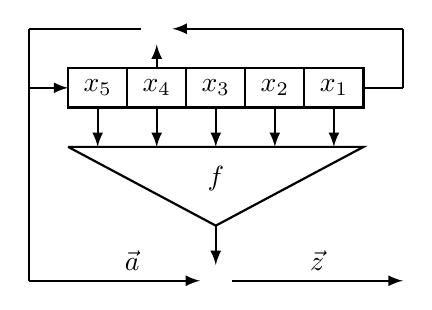
\begin{tikzpicture}[>=latex]
{\centering

\foreach \i in  {0,...,4}{
	\pgfmathtruncatemacro{\n}{5 - \i}
	\draw[thick] (\i * 0.75, 0) rectangle node[midway] {$x_\n$} (\i * 0.75 + 0.75, 0.5);
    \draw[thick, ->] (0.375 + \i * 0.75, 0) -- (0.375 + \i * 0.75, -0.5);
}

\draw[thick, <-] (0,0.25) -- (-0.5,0.25);
\draw[thick, -] (-0.5, -2.2) -- (-0.5,1);
\draw[thick, -] (-0.5,1) -- (0.925,1);

\xor{1.125}{1}{0.2}

\draw[thick, -] (3.75, 0.25) -- (4.25,0.25);
\draw[thick, -] (4.25, 0.25) -- (4.25,1);
\draw[thick, <-] (1.325,1) -- (4.25,1);
\draw[thick, ->] (1.125, 0.5) -- (1.125, 0.8);

\draw[thick, -] (0, -0.5) -- (3.75, -0.5) -- (1.875, -1.5) -- (0, -0.5);
\draw (1.875, -0.9) node {$f$};

\draw[thick, ->] (1.875, -1.5) -- (1.875, -2);

\xor{1.875}{-2.2}{0.2}

\draw[thick, ->] (-0.5, -2.2) -- node[above right] {$\vec{a}$} (1.675, -2.2);
\draw[thick, ->] (2.075, -2.2) -- node[above] {$\vec{z}$} (4.25, -2.2);
}
\end{tikzpicture}
}

Проведём расчёт метода. Длина вектора $\vec{z}$: $N = 31$. Длина ЛРС: $r = 5$. Количество слагаемых в линейной рекурренте: $t=2$. Вероятность того, что функция усложнения будет равна нулю: $P(f=0) = \frac{3}{4}$. Поскольку эта вероятность $\approx 75\%$, можно эффективно применить корреляционную атаку Мейера-Штаффельбаха (алгоритм A) \footnote{Meier, W., Staffelbach, O.: Fast correlation attacks on certain stream ciphers. J. Cryptol. 1(3),
159–176 (1989)}. Необходимое количество уравнений в системе: $m \approx (t + 1) \left[ \log_2{\frac{N}{r}} \right] = 6$.

Получим линейную рекурренту генератора:
$$a_{n+r} = a_n + a_{n+3}$$

Заменой $n+r$ и $n+3$ на $n$ дополнительно получим 2 уравнения:

\begin{equation*}
\begin{cases}
a_n = a_{n+r} + a_{n+3}, \\
a_n = a_{n-r} + a_{n-r+3}, \\
a_n = a_{n-3} + a_{n+r-3}.
\end{cases}
\end{equation*}

Подставим $a_{n+r}$ из первого уравнения вместо $a_{n-r}$ во второе уравнение и $a_{n+3}$ вместо $a_{n-3}$ в третье.

\begin{equation*}
\begin{cases}
a_n = a_{n+r} + a_{n+3},\ (1) \\
a_n = a_{n-r} + a_{n-r+3},\ (2) \\
a_n = a_{n-3} + a_{n+r-3},\ (3) \\
a_n = a_{n-2r} + a_{n-2r+3} + a_{n-r+3},\ (1+2) \\
a_n = a_{n-6} + a_{n+r-6} + a_{n+r-3}.\ (1+3)
\end{cases}
\end{equation*}

Теперь подставим второе уравнение в пятое.

\begin{equation*}
\begin{cases}
a_n = a_{n+r} + a_{n+3},\ (1) \\
a_n = a_{n-r} + a_{n-r+3},\ (2) \\
a_n = a_{n-3} + a_{n+r-3},\ (3) \\
a_n = a_{n-2r} + a_{n-2r+3} + a_{n-r+3},\ (1+2) \\
a_n = a_{n-6} + a_{n+r-6} + a_{n+r-3}.\ (1+3) \\
a_n = a_{n-r-6} + a_{n-r-3} + a_{n+r-6} + a_{n+r-3}.\ (1+2+3)
\end{cases}
\end{equation*}

Таким образом, мы получили систему из $m=6$ уравнений. Теперь подставим $r$, вместо членов последовательности $a$ подставим члены последовательности $z$, опустим индексы $n$ и получим систему линейных форм:

\begin{equation*}
\begin{cases}
z + z_{5} + z_{3} = L_1, \\
z + z_{-5} + z_{-2} = L_2, \\
z + z_{-3} + z_{2} = L_3, \\
z + z_{-10} + z_{-7} + z_{-2} = L_4, \\
z + z_{-6} + z_{-1} + z_{2} = L_5, \\
z + z_{-11} + z_{-8} + z_{-1} + z_{2} = L_6.
\end{cases}
\end{equation*}

Каждый $z_i$ представляет собой $a_i \oplus \gamma_i$, где $\gamma_i$ -- это н.о.р.с.в. \\ с $P(\gamma = 0) = P(f = 0) = \frac{3}{4}$. Пусть $b_{ij}$ -- это слагаемые правой стороны уравнений системы с $a_i$, а $y_{ij}$ -- слагаемые левой стороны уравнений системы с $z_i$, не содержащие $z$. Тогда уравнения первой системы принимают вид $a + \sum_{j=0}^{t}b_{ij} = 0$, а второй -- $z + \sum_{j=0}^{t}y_{ij} = L_i$. Заметим, что в таком случае $P(z_i = a_i) = P(y_{ij} = b_{ij}) = \frac{3}{4} = p$.

Пусть вероятность $s = s(t, p) = P(y_i = b_i)$ не зависит от $i$. По формуле полной вероятности получим рекуррентное соотношение:

\begin{equation*}
\begin{cases}
s(t,p) = p \cdot s(t-1, p) + (1-p)(1-s(t-1, p)), \\
s(1,p) = p.
\end{cases}
\end{equation*}

Поскольку $t=2$, то $s = s(2, \frac{3}{4}) = \frac{3}{4} \cdot \frac{3}{4} + (1-\frac{3}{4})(1-\frac{3}{4}) = \frac{5}{8}$. Определим апостериорную вероятность того, что $z=a$ при условии события $B_k$: $k$ из $m$ линейных форм $L_i$ равны нулю.
$$P(z=a|B_k) = \frac{\binom{m}{k} p s^k (1-s)^{m-k}}{\binom{m}{k} p s^k (1-s)^{m-k} + \binom{m}{k} (1-p) s^{m - k} (1-s)^k} = p^*$$

Найдём матожидания этой величины в двух разных случаях: $z=a$ и $z \ne a$:
\begin{multline*}
E_0 (p^*) = E(p^*|z=a) = \\ = \sum_{k=0}^{m} \binom{m}{k} \frac{p s^k (1-s)^{m-k}}{p s^k (1-s)^{m-k} + (1-p) s^{m - k} (1-s)^k} s^k (1-s)^{m-k} = \\
= \sum_{k=0}^{6} \binom{6}{k} \frac{\frac{3}{4} \cdot (\frac{5}{8})^k (\frac{3}{8})^{6-k}}{\frac{3}{4} \cdot (\frac{5}{8})^k (\frac{3}{8})^{6-k} + \frac{1}{4} \cdot (\frac{5}{8})^{6 - k} (\frac{3}{8})^k} \left( \frac{5}{8} \right)^k \left( \frac{3}{8} \right)^{6-k} \approx 0.81
\end{multline*}
\begin{multline*}
E_1 (p^*) = E(p^*|z \ne a) = \\ = \sum_{k=0}^{m} \binom{m}{k} \frac{p s^k (1-s)^{m-k}}{p s^k (1-s)^{m-k} + (1-p) s^{m - k} (1-s)^k} s^{m-k} (1-s)^k = \\
= \sum_{k=0}^{6} \binom{6}{k} \frac{\frac{3}{4} \cdot (\frac{5}{8})^k (\frac{3}{8})^{6-k}}{\frac{3}{4} \cdot (\frac{5}{8})^k (\frac{3}{8})^{6-k} + \frac{1}{4} \cdot (\frac{5}{8})^{6 - k} (\frac{3}{8})^k} \left( \frac{5}{8} \right)^{6-k} \left( \frac{3}{8} \right)^{k} \approx 0.56
\end{multline*}

Составим таблицу в соответствии с последней системой. Записываем последовательность $z$ в том же порядке, в котором она была задана в условии. Далее добавляем столбцы $z_i$, участвующие в СЛАУ в качестве слагаемых: это будет та же последовательность, но со сдвигом $i$. $i$ положительное -- сдвиг "вверх", $i$ отрицательное -- сдвиг "вниз". Потом заполняем $L_i$, исходя из их равенств, уже зная все слагаемые в них.

\medskip

\begin{adjustbox}{center}
\begin{tabular}{||c|c|c|c|c|c|c|c|c|c|c|c|c|c|c|c|c|c|c|c||}
\hline
$N$ & $z$ & $z_5$ & $z_3$ & $z_{-5}$ & $z_{-2}$ & $z_{-3}$ & $z_{2}$ & $z_{-10}$ & $z_{-7}$ & $z_{-6}$ & $z_{-1}$ & $z_{-11}$ & $z_{-8}$ & $L_1$ & $L_2$ & $L_3$ & $L_4$ & $L_5$ & $L_6$\\
\hline
1 & 0 & 1 & 1 & 0 & 0 & 0 & 0 & 1 & 1 & 0 & 0 & 0 & 1 & 0 & 0 & 0 & 0 & 0 & 1 \\
\hline
2 & 1 & 1 & 0 & 1 & 0 & 0 & 1 & 1 & 0 & 0 & 0 & 1 & 1 & 0 & 0 & 0 & 0 & 0 & 0 \\
\hline
3 & 0 & 0 & 1 & 0 & 0 & 0 & 0 & 1 & 0 & 1 & 1 & 1 & 0 & 1 & 0 & 0 & 1 & 0 & 0 \\
\hline
4 & 1 & 1 & 1 & 0 & 1 & 0 & 1 & 1 & 1 & 0 & 0 & 1 & 0 & 1 & 0 & 0 & 0 & 0 & 1 \\
\hline
5 & 0 & 1 & 0 & 0 & 0 & 1 & 1 & 0 & 0 & 0 & 1 & 1 & 1 & 1 & 0 & 0 & 0 & 0 & 0 \\
\hline
6 & 1 & 1 & 1 & 0 & 1 & 0 & 0 & 0 & 0 & 0 & 0 & 0 & 0 & 1 & 0 & 1 & 0 & 1 & 1 \\
\hline
7 & 1 & 1 & 1 & 1 & 0 & 1 & 1 & 1 & 0 & 0 & 1 & 0 & 0 & 1 & 0 & 1 & 0 & 1 & 1 \\
\hline
8 & 0 & 0 & 1 & 0 & 1 & 0 & 1 & 0 & 0 & 1 & 1 & 1 & 0 & 1 & 1 & 1 & 1 & 1 & 1 \\
\hline
9 & 1 & 0 & 1 & 1 & 1 & 1 & 1 & 0 & 1 & 0 & 0 & 0 & 0 & 0 & 1 & 1 & 1 & 0 & 0 \\
\hline
10 & 1 & 1 & 0 & 0 & 0 & 1 & 1 & 0 & 0 & 1 & 1 & 0 & 1 & 0 & 1 & 1 & 1 & 0 & 0 \\
\hline
11 & 1 & 1 & 0 & 1 & 1 & 0 & 0 & 0 & 1 & 0 & 1 & 0 & 0 & 0 & 1 & 1 & 1 & 0 & 0 \\
\hline
12 & 1 & 0 & 1 & 1 & 1 & 1 & 0 & 1 & 0 & 1 & 1 & 0 & 1 & 0 & 1 & 0 & 1 & 1 & 1 \\
\hline
13 & 0 & 0 & 1 & 0 & 1 & 1 & 1 & 0 & 1 & 1 & 1 & 1 & 0 & 1 & 1 & 0 & 0 & 1 & 1 \\
\hline
14 & 0 & 0 & 0 & 1 & 1 & 1 & 1 & 1 & 1 & 0 & 0 & 0 & 1 & 0 & 0 & 0 & 1 & 1 & 0 \\
\hline
15 & 1 & 1 & 0 & 1 & 0 & 1 & 0 & 0 & 0 & 1 & 0 & 1 & 1 & 0 & 0 & 0 & 1 & 0 & 1 \\
\hline
16 & 1 & 0 & 0 & 1 & 0 & 0 & 0 & 1 & 1 & 1 & 1 & 0 & 0 & 1 & 0 & 1 & 1 & 1 & 0 \\
\hline
17 & 0 & 1 & 1 & 1 & 1 & 0 & 0 & 1 & 1 & 1 & 1 & 1 & 1 & 0 & 0 & 0 & 1 & 0 & 1 \\
\hline
18 & 0 & 1 & 0 & 0 & 1 & 1 & 1 & 0 & 1 & 1 & 0 & 1 & 1 & 1 & 1 & 0 & 0 & 0 & 1 \\
\hline
19 & 0 & 1 & 1 & 0 & 0 & 1 & 0 & 1 & 1 & 0 & 0 & 0 & 1 & 0 & 0 & 1 & 0 & 0 & 1 \\
\hline
20 & 1 & 1 & 1 & 1 & 0 & 0 & 1 & 1 & 0 & 0 & 0 & 1 & 1 & 1 & 0 & 0 & 0 & 0 & 0 \\
\hline
21 & 0 & 0 & 1 & 1 & 0 & 0 & 1 & 1 & 0 & 1 & 1 & 1 & 0 & 1 & 1 & 1 & 1 & 1 & 1 \\
\hline
22 & 1 & 0 & 1 & 0 & 1 & 0 & 1 & 1 & 1 & 1 & 0 & 1 & 0 & 0 & 0 & 0 & 0 & 1 & 1 \\
\hline
23 & 1 & 1 & 0 & 0 & 0 & 1 & 1 & 0 & 1 & 0 & 1 & 1 & 1 & 0 & 1 & 1 & 0 & 1 & 1 \\
\hline
24 & 1 & 0 & 0 & 0 & 1 & 0 & 0 & 0 & 0 & 0 & 1 & 0 & 1 & 1 & 0 & 1 & 0 & 0 & 1 \\
\hline
25 & 1 & 0 & 1 & 1 & 1 & 1 & 0 & 1 & 0 & 0 & 1 & 0 & 0 & 0 & 1 & 0 & 1 & 0 & 0 \\
\hline
26 & 0 & 0 & 0 & 0 & 1 & 1 & 1 & 1 & 0 & 1 & 1 & 1 & 0 & 0 & 1 & 0 & 0 & 1 & 1 \\
\hline
27 & 0 & 0 & 0 & 1 & 1 & 1 & 0 & 0 & 1 & 0 & 0 & 1 & 0 & 0 & 0 & 1 & 0 & 0 & 1 \\
\hline
28 & 1 & 1 & 0 & 1 & 0 & 1 & 0 & 0 & 0 & 1 & 0 & 0 & 1 & 0 & 0 & 0 & 1 & 0 & 0 \\
\hline
29 & 0 & 0 & 0 & 1 & 0 & 0 & 0 & 0 & 1 & 1 & 1 & 0 & 0 & 0 & 1 & 0 & 1 & 0 & 1 \\
\hline
30 & 0 & 1 & 1 & 1 & 1 & 0 & 0 & 1 & 1 & 1 & 0 & 0 & 1 & 0 & 0 & 0 & 1 & 1 & 1 \\
\hline
31 & 0 & 0 & 0 & 0 & 0 & 1 & 1 & 0 & 1 & 1 & 0 & 1 & 1 & 0 & 0 & 0 & 1 & 0 & 1 \\
\hline
\end{tabular}
\end{adjustbox}

\medskip

Выберем $r$ строк, в которых $L_i$ принимают наибольшее количество нулей. Это строки 2, 1, 5, 20, 28. Выразим $a$ с соответствующими номерами через начальное заполнение регистров.

\begin{equation*}
\begin{cases}
a_2 = x_2 + x_5 = 1, \\
a_1 = x_1 + x_4 = 0, \\
a_5 = x_1 + x_3 + x_4 + x_5 = 0, \\
a_{20} = x_3 + x_4 + x_5 = 1, \\
a_{28} = x_2 = 1.
\end{cases}
\end{equation*}

Решив систему уравнений, получим $\vec{x} = (1, 1, 0, 1, 0)$. Выполним проверку:

\begin{lstlisting}
>>> def check_solution(x):
... 	true_z = [int(c) for c in '0101011011110011000101111001000']
... 	z = []
... 	for i in range(len(true_z)):
... 		gamma = x[3] * x[4]
... 		a = (x[0] + x[3]) % 2
... 		z += [(gamma + a) % 2]
... 		x = x[1:] + [a]
... 	return z == true_z
... 
>>> x = [1, 1, 0, 1, 0]
>>> check_solution(x)
False
\end{lstlisting}

К сожалению, не повезло. Значит, надо выбрать другие строки. Попробуем взять 2, 1, 5, 3, 28. Тогда четвёртое уравнение в системе изменится на $a_3 = x_1 + x_3 + x_4 = 0$. Новая система будет иметь два решения: $\vec{x} = (0, 1, 0, 0, 0)$ и $\vec{x} = (1, 1, 0, 1, 0)$. Второе из них уже было проверено выше, проверим первое:

\begin{lstlisting}
>>> x = [0, 1, 0, 0, 0]
>>> check_solution(x)
True
\end{lstlisting}

Победа.

Ответ: $m = 6$, $E_0 (p^*) \approx 0.81$, $E_1 (p^*) \approx 0.56$, $\vec{x} = (0, 1, 0, 0, 0)$.
